% ---------------------------------------------
%  describe document
% ---------------------------------------------

\documentclass[12pt
               % , final % turn on ``final'' to hide to-do bubbles
              ]{article}



% --- type, text, math, in/out encoding -----------------------

% This section is kinda non-essential
% These packages control typography, typeface, and input/output characters.
% The inputenc and fontenc pkgs may be important for non-English text,
%   but the rest are fluff.

\usepackage{microtype} % microtypographical things (not essential)

% fonts: 
\usepackage{mathptmx}       % serif = times (with math fonts!)
\usepackage{helvet}         % sans-serif = helvetica clone
\usepackage[varqu]{zi4}     % mono = inconsolata

% if you write non-English or need special accent characters, load these
\usepackage[utf8]{inputenc} % better interpretation of input characters
\usepackage[T1]{fontenc}    % better output glyphs/behaviors


% --- Margins and Spacing -----------------------

\usepackage[margin = 1.25in]{geometry} %margins % ipad geometry is 4X3
\usepackage{setspace} % line spacing
\usepackage{enumitem} % list settings
  \setlist{noitemsep} % (no separation between list items)


% --- math --------------------------------

\usepackage{amsmath} % math functions
\usepackage{amssymb} % math symbols


% --- tables and figures -----------------------

\usepackage{graphicx} % input graphics
\usepackage{float} % only good for H float option?
\usepackage{placeins} % for \FloatBarrier
\usepackage{booktabs} %? for toprule, midrule etc
\usepackage{dcolumn} % decimal-aligned columns



% --- document logic and utilities -----------------------

% ! not ``essential'' but handy enough to include

% hyperlinks and link colors
\usepackage{hyperref} 
\hypersetup{colorlinks = true, 
            citecolor = black, linkcolor = violet, urlcolor = teal}

% to-do notes
\usepackage[colorinlistoftodos, 
            prependcaption, 
            obeyFinal,
            textsize = footnotesize]{todonotes}
  \presetkeys{todonotes}{fancyline, color = violet!30}{}

% block comments
\usepackage{comment}





% --- References -----------------------

% you will need to change the path to the bib file
\usepackage[authordate, backend = biber]{biblatex-chicago}
\addbibresource{bib/workflow-bib.bib}



% --- global title/section formatting -----------------------

% ! also non-essential
% These are aesthetic tweaks to the abstract and section title design.
% You may want to delete these if you don't like.

% abstract settings
\usepackage{abstract}
\renewcommand{\abstractname}{}    % abstractname replaced with NULL
\renewcommand{\absnamepos}{empty} % removes the block where abstract would
                                  %   have been placed, originally 'center'

% section title settings
\usepackage[rm, small, sc]{titlesec} % titles are non-bold, small, caps
\titleformat*{\subsection}{\itshape} % subsection titles are italic
\titleformat*{\paragraph}{\itshape}  % paragraph titles are italic







% --- fancy code blocks -----------------------

% WARNING to workshop participants:
% These ``listings'' settings are included to make code blocks prettier,
%   but ``listings'' is inessential unless you want to make pretty code blocks,
%   which should be rare unless you're describing computer algorithms.
% I would NOT paste these settings into your future work.

% If you're interested in printing code, you might also check out ``minted''.
% Minted prints prettier code blocks, 
% but it depends on pygments (http://pygments.org/) which can be a pain

\usepackage{listings}

\definecolor{lgray}{gray}{0.925}

\lstset{ 
  backgroundcolor = \color{lgray},
  basicstyle = \ttfamily, % code style
  breakatwhitespace = true,      % if automatic break only happen at whitespace
  breaklines = false,            % automatic line breaking
  columns=fullflexible,          % kerning thing
  commentstyle = \color{gray},   % comment style
  escapeinside = {\% *}{*)},     % for using LaTeX within code
  keepspaces = true,             % keeps spaces for indentation 
                                 % (needs columns = flexible ?)
  language = TeX,                % the language of the code
  % morekeywords = {*,...},        % for adding more keywords
  showstringspaces = false      % underline spaces within strings only
}






% ----------------------------------------------------
%   writing
% ----------------------------------------------------


\begin{document}


\title{{\LaTeX} Workflow Demonstration}
\author{Michael G.\ DeCrescenzo%
          \thanks{Ph.D.\ Candidate, Political Science, University of Wisconsin--Madison.}}
\date{Updated \today}
\maketitle


\begin{abstract}
  This document describes how to incorporate {\LaTeX} into a social science workflow. It covers bibliographies (using Bib{\LaTeX}) and integration with statistical software (tables, figures, and ``saved quantities''). The bibliography is managed by a companion \texttt{workflow.bib} file. The software integration component focuses primarily on \texttt{R}, but the same concepts generally apply to Stata. All tables and figures are created algorithmically to maximize reproducibility throughout the workflow. All of the technological capabilities demonstrated in this document are possible using RMarkdown, with a demonstration contained in a separate folder in the online repository.%
    \footnote{\url{https://github.com/mikedecr/latex-workshop-2018}}
  Slideshows using \texttt{Beamer} are also discussed in a separate folder. 
\end{abstract}



\onehalfspacing


\section{Introduction: The value of {\LaTeX}}

{\LaTeX} is designed to emphasize content control over aesthetic micromanagement. This document exemplifies how far ``content control'' goes. It covers much more than just managing \emph{variables} about the document itself, such as the title, author name, margin sizes, and so on. It extends to more advanced topics that can be automated: bibliographies, tables, figures, and other aspects of your empirical results.

Many {\LaTeX} hop off the train before learning these skills. They know how to create {\LaTeX} documents, but they don't fully learn how to manage bibliographies or integrate their statistical output with their \texttt{.tex} files. These people are selling themselves short! Dig into the source code of this document to learn more.


\section{Bibliographies}

{\LaTeX} lets you automate the formatting of (a) in-text citations and (b) their corresponding bibliography entries in the back of your paper. 

How? First, create a \texttt{.bib} file. A \texttt{bib} file contains information about works you would like to cite---the author, date, title, journal, volume and issue number, and so on. An example \texttt{bib} file is included with this document, so you can see how the syntax works. 

Each entry in the \texttt{bib} file has a \emph{cite key}, which is a short string of unique text that serves as a label for each entry. When you are writing your document, you refer to the cite key to import information about the referenced work.

\subsection{Bibliography systems}

You may read about different bibliography systems and packages. To learn more, follow the link in this footnote.%
  \footnote{\url{https://tex.stackexchange.com/a/25702}}
Here's a short version:
\begin{itemize}
 \item There are two common back-end systems you could choose from: \texttt{bibtex} and \texttt{biber}. These systems interface between your \texttt{bib} file and your \texttt{tex} file. We will use \texttt{biber} because it is more flexible, powerful, and actively developed.
 \item There are two front-end bibliography packages you could choose from: \texttt{natbib} and \texttt{biblatex}. They are (loosely speaking) companions to \texttt{bibtex} and \texttt{biber}, respectively. They control the commands you use to summon and customize the appearance of your citations.
\end{itemize}

We will use a combination of \texttt{biber} and \texttt{biblatex}, because they're a bit simpler. Luckily, changing between systems is not too challenging, should you find that you need to modify your citation system.%
  \footnote{You can view \texttt{natbib}/\texttt{bibtex} instructions in last year's workshop: \url{https://github.com/mikedecr/latex-workshop/blob/master/slides-2-bibs/latex-workshop-bib-slides.pdf}. Thomas Leeper has an APSA-formatted bibliography style file for use with \texttt{natbib} here: \url{https://github.com/leeper/apsa-leeper.bst/blob/master/apsa-leeper.bst}}
The following code sits in the preamble:
\newline
\begin{minipage}{\linewidth}
\begin{lstlisting}
  \usepackage[authordate, backend = biber]{biblatex-chicago} 
  \addbibresource{bib/workflow-bib.bib}
\end{lstlisting}
\end{minipage}
The first line calls the \texttt{biblatex} package using Chicago style (very similar to APSA style), and the second line defines the pathway to your \texttt{.bib} file. In the body of your document, insert the bibliography section using \verb+\printbibliography+.




\subsection{Citation commands}

When you read a paper, you encounter citations of various formats. This section describes how to create those citation formats yourself, using Bib{\LaTeX} syntax.

\paragraph{Textual citations} 
``Text'' citations are citations where we refer directly to an article in the text. For example, not every statistical estimate is statistically significant, but \textcite{Gelman2006significance} point out that statistically significant and insignificant estimates are sometimes similar to one another. This is done using \verb+\textcite{citekey}+: 
\newline
\begin{minipage}{\linewidth}
\begin{lstlisting}
  not every statistical estimate is statistically significant, 
  but \textcite{Gelman2006significance} point out...
\end{lstlisting}
\end{minipage}

\paragraph{Parenthetical citations} 
The difference between ``significant'' and ``insignificant'' is not itself significant \parencite{Gelman2006significance}. This is done using \verb+\parencite{citekey}+.

\paragraph{``Plain'' citations} 
This citation is inserted with no parentheses whatsoever. As it happens, this is most useful when you are \emph{already within} parentheses. For example, not all of our estimates are significant, but the insignificant estimates are of a similar magnitude to the significant estimates (see e.g.\ \cite{Gelman2006significance}). Do this using \verb+\cite{citekey}+.

\paragraph{Footnote citations}
If you are an international relations scholar, you are more likely to deal with the journal \emph{International Organization}, which famously uses footnote citations. You can make these with \verb+\footcite{citekey}+. Remember, footnotes go \emph{after} punctuation. Some people said something about statistical significance once.\footcite{Gelman2006significance}
\newline
\begin{minipage}{\linewidth}
\begin{lstlisting}
  Some people said something about statistical 
  significance once.\footcite{Gelman2006significance}
\end{lstlisting}
\end{minipage}


\paragraph{Invisible citations}
If you want to include a bibliography entry, but you have no reason to include an in-text citation, you can use \verb+\nocite{citekey}+. The entry appears in the bibliography, but nothing else appears in the text. (You will notice a Gelman piece about multilevel modeling in the bibliography.) This is often handy for citing software or data that you rely on. \nocite{Gelman2006multilevel}


\subsection{Tools for easier bibliographies}

How do you get bibliographic information into your \texttt{.bib} file?

\paragraph{Hand-typing} Enter bibliographic information by hand \emph{if you have to}, but there are probably tools that make the process easier.

\paragraph{Google Scholar} 
Google Scholar has a citation button that lets you access citations in multiple formats. Just click the \texttt{''} button and ask for Bib{\TeX} format\ldots
  \begin{center}
    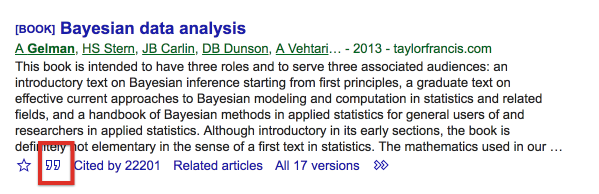
\includegraphics[width = 0.9\textwidth]{graphics/scholar.png}
  \end{center}
\ldots and it will give you some text that you can copy into your \texttt{.bib} file.

\paragraph{Google Scholar Button} Google offers a web extension called the \emph{Google Scholar Button}, which gives you a menu-bar button to search and collect info using Google Scholar. 
\begin{center}
  
\includegraphics[width = 0.7\textwidth]{graphics/scholar-button.png}
\end{center}

\paragraph{DOI Numbers} Get bibliographic info from DOI numbers using \url{doi2bib.org} is simple. Paste a DOI number, get a \texttt{.bib} entry.


\paragraph{Mendeley, Zotero, BibDesk\ldots} There are a handful of reference-manager apps. You can get these apps to export \texttt{.bib} entries for the works in your library.

\paragraph{Various R packages} There are some \texttt{R} packages out there that provide package utilities, such as importing all entries from a \texttt{.bib} file into a data frame for customization within \texttt{R}.%
  \footnote{\url{https://cran.r-project.org/web/packages/bib2df/vignettes/bib2df.html}}



\subsection{Bibliography tips}

One tip I have for using {\LaTeX} for bibliographies is to keep a global \texttt{.bib} file somewhere on your computer. I keep mine in my synced \texttt{Dropbox} folder so it is always backed up online. You could keep yours in a \texttt{git} repository with a remote backup. Whichever works. Keeping a global \texttt{.bib} file makes it easy to include references in whatever you're working on. 

\emph{However.} However, however, however. If you want your project to be \emph{reproducible}, you should eventually have a local, project-specific \texttt{.bib} file by the time you are distributing your project anywhere (to coauthors, to journals, etc). This ensures that your project repository is always reproducible as a folder unto itself. 

There is other great advice on the web.%
  \footnote{\url{https://serialmentor.com/blog/2015/10/2/Bibtex}}
 




\section{Tables}

As last week's \texttt{handout} document showed, tables are weird in {\LaTeX}. They make syntactic sense, but the syntax itself is complicated and prone to user error. The beauty of {\LaTeX}, however, is that its \emph{content control} capabilities obviate the necessity to create tables by hand in almost every instance. You can have \texttt{R} or \texttt{Stata} do that for you.

The online repository for this workshop contains a folder of \texttt{R} code. In it, you can find a \texttt{workflow.R} file to accompany this document. It discusses how to create {\LaTeX} tables algorithmically. It works generally like this:
\begin{enumerate}
 \item Do some analysis in \texttt{R} or \texttt{Stata}.
 \item Create a table. 
 \item Convert the table to \texttt{.tex} code; save the \texttt{tex} table in a separate \texttt{.tex} file.%
   \footnote{The \texttt{R} script uses a few different packages for exporting tables. Stata code generally relies on the \texttt{outtex} package for exporting tables as {\LaTeX} code.}
 \item In your main \texttt{tex} file, import the \texttt{tex} file for the table.%
   \footnote{Yes, you can import \texttt{tex} documents into other \texttt{tex}documents. This can actually be very handy for managing large projects such as books or, ahem, dissertations.}
\end{enumerate}
We will see this in action using some Pok\'emon data.%
  \footnote{\emph{For the record}, I am not a Pok\'emon fanatic, but this is a fun dataset.}

\subsection{An \texttt{xtable} example}

My preferred package for outputting summary statistics from \texttt{R} to {\LaTeX} is the \texttt{xtable} package. It straightforwardly converts data frames into nicely formatted tables with sensible options. 

The \texttt{R} file processes the data, creates a table in \texttt{tex} code, and saves the table in the file \texttt{pokemon-stats.tex} (within the \texttt{tables} subfolder). To import the table, I write\ldots
\newline
\begin{minipage}{\linewidth}
\begin{lstlisting}
  % latex table generated in R 3.5.0 by xtable 1.8-2 package
% Wed Sep 19 16:14:59 2018
\begin{table}[ht]
\centering
\begin{tabular}{rrrrrrr}
  \toprule
Generation & HP & Attack & Defense & Sp. Atk & Sp. Def & Speed \\ 
  \midrule
1 & 66 & 77 & 71 & 72 & 69 & 73 \\ 
  2 & 71 & 72 & 73 & 66 & 74 & 62 \\ 
  3 & 67 & 82 & 74 & 76 & 71 & 67 \\ 
  4 & 73 & 83 & 78 & 76 & 77 & 71 \\ 
  5 & 72 & 82 & 72 & 72 & 69 & 68 \\ 
  6 & 68 & 76 & 77 & 74 & 75 & 66 \\ 
   \bottomrule
\end{tabular}
\caption{Mean Pok\'emon Statistics} 
\label{tab:pm}
\end{table}


\end{lstlisting}
\end{minipage}
\ldots which tells {\LaTeX} to import any code that lives in the \texttt{tables/pokemon-stats.tex} file. It happens to contain a table, so a table is produced. Because the table is contained in a \texttt{float} environment, it may not appear right here in the PDF, but it will be somewhere sensible. I can refer to it with the label I created for it (in \texttt{R}) as Table~\ref{tab:pm}.

% latex table generated in R 3.5.0 by xtable 1.8-2 package
% Wed Sep 19 16:14:59 2018
\begin{table}[ht]
\centering
\begin{tabular}{rrrrrrr}
  \toprule
Generation & HP & Attack & Defense & Sp. Atk & Sp. Def & Speed \\ 
  \midrule
1 & 66 & 77 & 71 & 72 & 69 & 73 \\ 
  2 & 71 & 72 & 73 & 66 & 74 & 62 \\ 
  3 & 67 & 82 & 74 & 76 & 71 & 67 \\ 
  4 & 73 & 83 & 78 & 76 & 77 & 71 \\ 
  5 & 72 & 82 & 72 & 72 & 69 & 68 \\ 
  6 & 68 & 76 & 77 & 74 & 75 & 66 \\ 
   \bottomrule
\end{tabular}
\caption{Mean Pok\'emon Statistics} 
\label{tab:pm}
\end{table}



The benefits of this system:
\begin{itemize}
 \item Except in very strange circumstances, there will be no need to hand-type your own {\LaTeX} tables again.
 \item If for any reason your results should change, the table will automatically be updated (in the \texttt{R} code), which will also update the \texttt{pokemon-stats.tex} file. As a result, the results in your {\LaTeX} document \emph{will always be up-to-date}. I cannot overstate how much of a big deal this is for your workflow.
\end{itemize}

Even if you want to create a table of textual information (no data), you can still use \texttt{R} to create it. The example in Table~\ref{tab:first-pm} uses a dataset containing only text variables to create a table of textual information. Again, I never touched {\LaTeX} to produce this table.

% latex table generated in R 3.5.0 by xtable 1.8-2 package
% Tue Sep 18 00:53:53 2018
\begin{table}[ht]
\centering
\begin{tabular}{llll}
  \toprule
Pok\'emon & Type & Weakness & Gary Picks \\ 
  \midrule
Bulbasaur & Grass & Fire & Charmander \\ 
  Squirtle & Water & Grass & Bulbasaur \\ 
  Charmander & Fire & Water & Squirtle \\ 
   \bottomrule
\end{tabular}
\caption{Choices for your first Pok\'emon} 
\label{tab:first-pm}
\end{table}





\subsection{Regression tables using \texttt{texreg}}

When exporting regression tables from \texttt{R}, I prefer the \texttt{texreg} package.%
  \footnote{The \texttt{stargazer} package is another popular choice for regression tables.} 
It can process a broad range of model types and has sensible options for regression output.

In the code, we estimate two models to predict a Pok\'emon's HP (``Hit points'', or \emph{health}) as a function of their Defense and Attack points. It seems sensible to me that Pok\'emon with low HP should be somewhat compensated with higher Defense capabilities. The regressions presented in Table~\ref{tab:pm-regs} so far contradict that intuition.


\begin{table}[ht]
\caption{Regressions predicting Pok\'emon HP}
\begin{center}
\begin{tabular}{l D{.}{.}{3.5} D{.}{.}{3.5} }
\toprule
 & \multicolumn{1}{c}{Restricted Model} & \multicolumn{1}{c}{Full Model} \\
\midrule
(Intercept) & 54.77^{***} & 40.77^{***} \\
            & (2.26)      & (2.46)      \\
Defense     & 0.20^{***}  & 0.06        \\
            & (0.03)      & (0.03)      \\
Attack      &             & 0.31^{***}  \\
            &             & (0.03)      \\
\midrule
R$^2$       & 0.06        & 0.18        \\
Adj. R$^2$  & 0.06        & 0.18        \\
Num. obs.   & 800         & 800         \\
RMSE        & 24.81       & 23.12       \\
\bottomrule
\multicolumn{3}{l}{\scriptsize{$^{***}p<0.001$, $^{**}p<0.01$, $^*p<0.05$}}
\end{tabular}
\label{tab:pm-regs}
\end{center}
\end{table}



\subsection{Other table tips}

If you want help creating {\LaTeX} and don't want to fuss with statistical code, here's what you can do.
\begin{itemize}
 \item I'll start by being pedantic: you should probably just learn to get comfortable with the statistical code. It's better for reproducibility and for reducing human error.
 \item \url{https://www.tablesgenerator.com/}
\end{itemize}


\section{Figures}

Figures follow a similar logic and rationale as tables. It's best to create them algorithmically in order to maximize the reproducibility of your project. Moreover, calling a figure file using {\LaTeX} ensures that your paper always has up-to-date results.

It's best to export graphics as \texttt{.pdf} files, which are ``vector'' graphics and thus are infinitely scalable without pixelation.

Figure~\ref{fig:type-reg} shows the effect of Pok\'emon type on their defense points (``Type'' is treated as a set of binary indicators with ``Bug'' as the omitted category). 

\begin{figure}[hbt]
 \begin{center}
 \caption{Effect of Pok\'emon ``Type'' on Defense Points (multilevel model)}
 \label{fig:type-reg}
 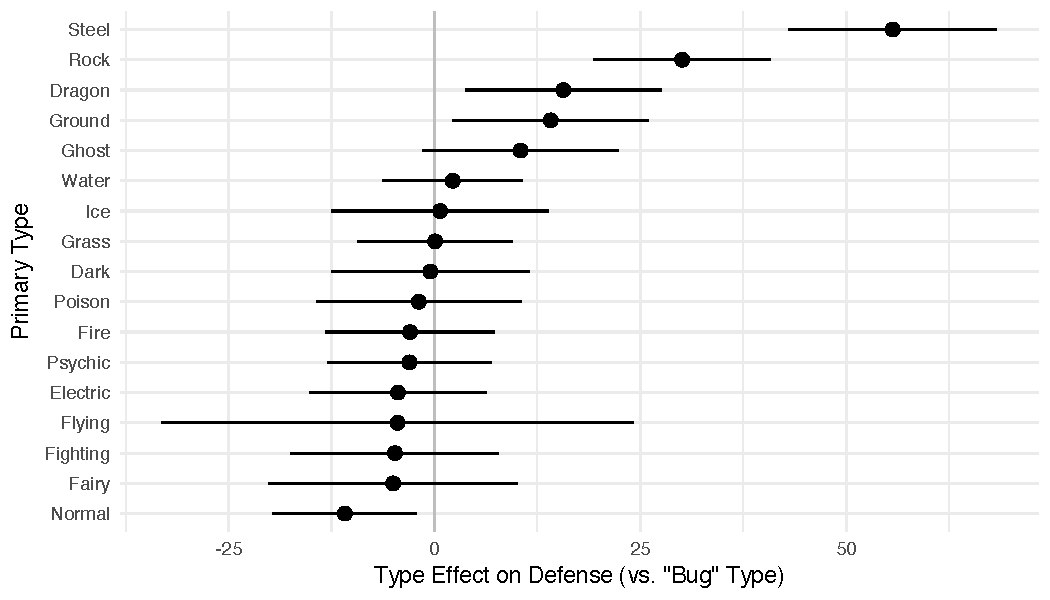
\includegraphics[width = \textwidth]{graphics/type-intercepts.pdf}
 \end{center}
\end{figure}



\section{Exported quantities}

Let's say that I wanted to refer to some exact quantities from my \texttt{R} results. I could type numbers in {\LaTeX} by hand, but that process is tedious and imprecise. Instead, I use \texttt{R} to save quantities directly into little \texttt{.tex} files, and then I pull those files into my paper using \verb+\input{}+.

For example, the only type that has a defense point value that is significantly \emph{lower} than ``Bug'' type is a ``Normal'' type Pok\'emon, with an effect of $-10.9
$ points ($p = 0.015
$).
\newline
\begin{minipage}{\linewidth}
\begin{lstlisting}
  with an effect of $-10.9
$ points 
  ($p = 0.015
$)
\end{lstlisting}
\end{minipage}
The largest difference compared to ``Bug'' type is ``Steel'' type, which has an average of $55.6
$ more defense points.
\newline
\begin{minipage}{\linewidth}
\begin{lstlisting}
   which has an average of $55.6
$ 
   more defense points
\end{lstlisting}
\end{minipage}




\section{Coda: Editing software}

An under-appreciated detail in your workflow is your code editing software. Different softwares offer different benefits---they won't all make your life easier in the same way.

An important detail for working with {\LaTeX} is \emph{auto-completion}---of your cite keys, file names, table and figure labels, and so on. Software like {\TeX}Maker provides these supports.

My own setup (Sublime Text with the {\LaTeX}Tools package) has additional capabilities with syntax highlighting, code snippets, and keybindings. As you grow more advanced in your use of {\LaTeX} and other coding languages, your preferences over these editor features may become more specific and refined. As always, I am happy to assist and advise on these choices.

I would enthusiastically recommend RStudio%
  \footnote{\url{https://www.rstudio.com/}}
to newcomers. Although Rstudio is designed as an \texttt{R} editor/IDE, it has capabilities for handling {\LaTeX}, Rmarkdown, and other languages that are valuable for social and data sciences.




\newpage
\printbibliography


\end{document}
